\documentclass[journal]{IEEEtran}
\usepackage[utf8]{inputenc}
\usepackage[spanish,es-tabla]{babel}
\usepackage{graphicx}
\usepackage{amsmath,amssymb}
\usepackage{booktabs}
\usepackage{cite}
\usepackage{tabularx}
\usepackage{multirow}
\usepackage{siunitx}
\usepackage{enumitem}
\usepackage{url}
\usepackage{microtype}

% Configuración de hipervínculos
\usepackage{hyperref}
\hypersetup{
    colorlinks=true,
    linkcolor=black,
    citecolor=black,
    urlcolor=blue
}

\begin{document}

\title{Monitoreo de Condición de un Sistema Hidráulico mediante Aprendizaje de Máquina: Extracción de Características y Clasificación Multiclase}

\author{
    \IEEEauthorblockN{Nelson Martín Villagra\IEEEauthorrefmark{1} y Víctor Hugo Astorga\IEEEauthorrefmark{2}} \\
    \IEEEauthorblockA{\textit{Especialización en Inteligencia Artificial (CEIA)} \\
    \textit{Facultad de Ingeniería, Universidad de Buenos Aires (FIUBA)} \\
    Ciudad Autónoma de Buenos Aires, Argentina \\
    Email: \IEEEauthorrefmark{1}nelsonmvillagra1976@gmail.com, \IEEEauthorrefmark{2}vhastorga@gmail.com}
    \thanks{Trabajo Práctico Final de la asignatura \emph{Aprendizaje de Máquina~I}, CEIA-FIUBA. Docente: Facundo Adrián Lucianna. Octubre de 2026.}
}

\maketitle

% ============================================================================
% RESUMEN
% ============================================================================
\begin{abstract}
El mantenimiento predictivo basado en la condición (\emph{Condition-Based Maintenance}, CBM) es un paradigma central en la Industria 4.0 para mitigar fallas imprevistas y reducir costos operativos en maquinaria pesada. En este trabajo se aborda el diagnóstico multiclase del estado de degradación de cuatro componentes críticos de un banco de pruebas hidráulico experimental (ZeMA): refrigerador (\emph{cooler}), válvula direccional, bomba volumétrica interna y acumulador hidráulico. A partir de las series temporales multivariadas registradas por 17~sensores físicos y virtuales con tasas de muestreo heterogéneas (\SI{1}{\hertz}, \SI{10}{\hertz} y \SI{100}{\hertz}), que suman 43\,680 atributos crudos por ciclo de trabajo de \SI{60}{\second}, se implementa una metodología de ingeniería de características que condensa cada ciclo en 204 descriptores estadísticos en el dominio temporal. 

Atendiendo rigurosamente a las recomendaciones sobre riesgo de fuga de información (\emph{data leakage}) derivadas del orden cronológico de las pruebas, se adopta un esquema de partición temporal estricto (75\% entrenamiento / 25\% evaluación), descartando la estratificación aleatoria no causal. Se formula un \emph{baseline} heurístico no algorítmico derivado de umbrales físicos del análisis exploratorio para contrastar cuatro familias de modelos de aprendizaje supervisado: K-Vecinos Más Cercanos (KNN), Máquinas de Vectores de Soporte (SVM), Árboles de Decisión y Ensambles (Random Forest y XGBoost), evaluados bajo métricas invariantes al desbalance (\emph{balanced accuracy} y \emph{F1-score macro}).
\end{abstract}

\begin{IEEEkeywords}
Mantenimiento Predictivo, Sistemas Hidráulicos, Aprendizaje de Máquina, Extracción de Características, Series Temporales, Data Leakage, Clasificación Multiclase.
\end{IEEEkeywords}

% ============================================================================
% 1. INTRODUCCIÓN
% ============================================================================
\section{Introducción}
\label{sec:intro}

\IEEEPARstart{E}{n} las instalaciones industriales modernas, los sistemas oleohidráulicos transmiten y controlan grandes densidades de potencia mecánica mediante fluidos presurizados. Por su propia naturaleza operativa, componentes como bombas de pistones, acumuladores de membrana, válvulas servo-direccionales e intercambiadores térmicos están sometidos a regímenes severos de fatiga mecánica, cavitación, erosión y degradación termo-oxidativa del fluido. Las estrategias tradicionales de mantenimiento correctivo (reparación posterior al fallo catastrófico) o preventivo sistemático (reemplazo ciego por horas de servicio acumuladas) conllevan pérdidas millonarias asociadas a paradas no programadas o sustitución prematura de componentes con vida residual útil~\cite{Helwig2015}.

El advenimiento del monitoreo de condición (\emph{Condition Monitoring System}, CMS) y el mantenimiento predictivo permite transicionar hacia intervenciones basadas exclusivamente en la evidencia cuantificable del estado del activo~\cite{Luong2019}. No obstante, la modelización analítica basada en primeros principios de sistemas multifísicos acoplados (hidráulica, térmica, eléctrica) resulta computacionalmente inviable o poco escalable ante desviaciones operacionales y ensuciamiento de sensores~\cite{Helwig2015b}. En este escenario, los métodos de aprendizaje automático (\emph{Machine Learning}, ML) aplicados a registros sensoriales multivariados ofrecen una alternativa robusta para inferir patrones de degradación incipientes~\cite{Schneider2017, Pedregosa2011}.

El presente estudio se centra en el banco de pruebas hidráulico desarrollado por ZeMA gGmbH y la Universidad del Sarre~\cite{Helwig2015}, disponible a través del repositorio académico de referencia UCI Machine Learning Repository~\cite{UCI_Dataset} y su réplica comunitaria en Kaggle~\cite{Kaggle_Dataset}. El sistema genera ciclos de trabajo de \SI{60}{\second} donde se inducen experimentalmente múltiples grados de fallo en cuatro componentes clave.

\subsection{Pregunta de investigación}

La formulación central que rige esta investigación se enuncia como:

\begin{quote}
\emph{¿Es factible determinar con alta precisión y reproducibilidad el grado de degradación multiclase de cuatro componentes hidráulicos individuales en ciclos de trabajo de \SI{60}{\second}, empleando exclusivamente descriptores estadísticos compactos extraídos de 17~señales de sensores continuos y evaluados bajo un esquema temporal estricto?}
\end{quote}

\subsection{Hipótesis de trabajo}

Con base en la termodinámica del banco y la literatura especializada~\cite{Helwig2015, Schneider2017}, se formulan cuatro hipótesis técnicas:

\begin{itemize}[leftmargin=*]
    \item \textbf{H1 (Refrigerador $\leftrightarrow$ Eficiencia y Temperatura):} Las variables virtuales de enfriamiento ($\text{CE}$ y $\text{CP}$) y las temperaturas del circuito ($\text{TS1}$--$\text{TS4}$) contienen información discriminante casi perfecta sobre la eficiencia del intercambiador de calor, permitiendo una clasificación separable mediante umbrales simples.
    \item \textbf{H2 (Válvula $\leftrightarrow$ Dinámica de Flujo y Presión):} La degradación del retardo de conmutación en la válvula direccional altera de forma mensurable las tasas de flujo transitorio ($\text{FS1}$, $\text{FS2}$) y la caída de presión en las líneas de trabajo ($\text{PS3}$, $\text{PS4}$).
    \item \textbf{H3 (Bomba y Acumulador $\leftrightarrow$ Potencia y Amortiguación):} Las pérdidas por fuga interna en la bomba principal y la descarga de nitrógeno en el acumulador se reflejan en la potencia eléctrica del motor ($\text{EPS1}$) y en la respuesta transitoria de las presiones de carga ($\text{PS5}$, $\text{PS6}$), aunque con menor separabilidad lineal debido a interferencias térmicas.
    \item \textbf{H4 (Jerarquía de Modelos y Ensambles):} Los clasificadores no lineales de ensamble (Random Forest y XGBoost) superarán a los métodos basados en distancias (KNN) y modelos lineales en los objetivos de alta complejidad (\emph{pump}, \emph{accumulator}), si bien un \emph{baseline} heurístico físico será competitivo en los componentes térmicamente desacoplados (\emph{cooler}).
\end{itemize}

\subsection{Alcance y definición del MVP}

Siguiendo las pautas metodológicas de la asignatura \emph{Aprendizaje de Máquina I} (CEIA--FIUBA), el proyecto se estructura bajo una estrategia iterativa:
\begin{enumerate}[leftmargin=*]
    \item \textbf{Producto Mínimo Viable (MVP):} Modelado y evaluación exhaustiva de los objetivos \emph{Cooler} (3 clases, balanceado) y \emph{Valve} (4 clases, desbalance moderado), comparando cuatro familias algorítmicas frente a un \emph{baseline} no algorítmico.
    \item \textbf{Objetivo Extendido (\emph{Stretch Goal}):} Extensión del pipeline verificado hacia los objetivos de conocida mayor dificultad reportada en la literatura: \emph{Internal pump leakage} y \emph{Hydraulic accumulator}~\cite{Helwig2015, Schneider2017}.
\end{enumerate}

% ============================================================================
% 2. DATOS Y FUENTE
% ============================================================================
\section{Datos y Fuente}
\label{sec:datos}

\subsection{Origen, trazabilidad y montaje experimental}

Los datos fueron obtenidos originalmente en el banco de pruebas experimental de ZeMA gGmbH (\emph{Zentrum für Mechatronik und Automatisierungstechnik}) y la Universidad del Sarre en Saarbrücken, Alemania~\cite{Helwig2015, Helwig2015b}. El conjunto fue donado formalmente al repositorio académico internacional \emph{UCI Machine Learning Repository}~\cite{UCI_Dataset} en abril de 2018 (donantes: M. Bastuck y T. Schneider), y se encuentra asimismo alojado como réplica pública exacta (\emph{mirror}) en la plataforma Kaggle~\cite{Kaggle_Dataset} (a través del cual fue descargado para este trabajo). Ambos repositorios comparten idéntica matriz de datos y documentación técnica original.

El banco físico consta de un circuito hidráulico primario de trabajo (bomba de pistones axiales accionada por motor de \SI{3.3}{\kilo\watt}, válvula direccional proportional, cilindro de carga y acumulador de amortiguación) y un circuito secundario de enfriamiento y filtrado de baja presión.

Durante 2\,205 ciclos continuos de \SI{60}{\second}, el sistema ejecuta una secuencia cíclica predefinida de aperturas y presurizaciones. En cada ciclo, se registran 17 magnitudes físicas y virtuales estructuradas en matrices tabuladas donde cada fila representa un ciclo completo.

\subsection{Heterogeneidad sensorial y dimensionalidad cruda}

A diferencia de datasets tabulares homogéneos, el conjunto de datos exhibe múltiples frecuencias de muestreo acordes con la constante de tiempo física del fenómeno monitoreado:
\begin{itemize}[leftmargin=*]
    \item \textbf{Presión y Potencia (\SI{100}{\hertz}):} Transitorios rápidos de apertura y conmutación de válvula ($6\,000$ muestras/ciclo por sensor).
    \item \textbf{Caudal volumétrico (\SI{10}{\hertz}):} Dinámica de flujo del circuito de trabajo ($600$ muestras/ciclo por sensor).
    \item \textbf{Temperatura y Vibración (\SI{1}{\hertz}):} Variables cuasi-estacionarias y virtuales ($60$ muestras/ciclo por sensor).
\end{itemize}

Como se resume en la Tabla~\ref{tab:sensors}, el número bruto de atributos por ciclo asciende a:
\begin{equation}
    D_{\text{crudo}} = 7 \times 6000 + 2 \times 600 + 8 \times 60 = 43\,680 \text{ atributos}
\end{equation}

\begin{table}[t]
    \centering
    \caption{Sensores e instrumentación del banco ZeMA~\cite{Helwig2015}.}
    \label{tab:sensors}
    \resizebox{\columnwidth}{!}{%
    \begin{tabular}{llccc}
        \toprule
        \textbf{Identificador} & \textbf{Magnitud Física} & \textbf{Unidad} & \textbf{Frecuencia} & \textbf{Atributos/Ciclo} \\
        \midrule
        PS1 -- PS6 & Presión circuito & \si{\bar} & \SI{100}{\hertz} & $6 \times 6\,000$ \\
        EPS1 & Potencia motor eléctrico & \si{\watt} & \SI{100}{\hertz} & $1 \times 6\,000$ \\
        FS1, FS2 & Caudal volumétrico & \si{\liter\per\minute} & \SI{10}{\hertz} & $2 \times 600$ \\
        TS1 -- TS4 & Temperatura fluido & \si{\degreeCelsius} & \SI{1}{\hertz} & $4 \times 60$ \\
        VS1 & Vibración mecánica & \si{\milli\meter\per\second} & \SI{1}{\hertz} & $1 \times 60$ \\
        CE & Eficiencia enfriamiento & \% & \SI{1}{\hertz} & $1 \times 60$ \\
        CP & Potencia enfriamiento & \si{\kilo\watt} & \SI{1}{\hertz} & $1 \times 60$ \\
        SE & Factor de eficiencia & \% & \SI{1}{\hertz} & $1 \times 60$ \\
        \midrule
        \textbf{Total} & \textbf{17 canales de medición} & & & \textbf{43\,680} \\
        \bottomrule
    \end{tabular}%
    }
\end{table}

\subsection{Variables objetivo (Targets)}

Las condiciones operativas se registraron ciclo a ciclo en el archivo \texttt{profile.txt}. En total se cuantifican cuatro fallas de componentes continuas (discretizadas en niveles) más una bandera de estabilidad térmica:

\begin{table}[t]
    \centering
    \caption{Distribución de clases en las variables objetivo.}
    \label{tab:targets}
    \resizebox{\columnwidth}{!}{%
    \begin{tabular}{lllcc}
        \toprule
        \textbf{Variable Target} & \textbf{Descripción Técnica} & \textbf{Clases} & \textbf{Instancias} & \textbf{Proporción} \\
        \midrule
        \multirow{3}{*}{\textbf{Cooler condition}} 
        & Falla casi total & 3\% & 732 & 33.2\% \\
        & Eficiencia reducida & 20\% & 732 & 33.2\% \\
        & Operación óptima & 100\% & 741 & 33.6\% \\
        \midrule
        \multirow{4}{*}{\textbf{Valve condition}} 
        & Conmutación óptima & 100\% & 1\,125 & 51.0\% \\
        & Retardo pequeño & 90\% & 360 & 16.3\% \\
        & Retardo severo & 80\% & 360 & 16.3\% \\
        & Falla total inminente & 73\% & 360 & 16.3\% \\
        \midrule
        \multirow{3}{*}{\textbf{Pump leakage}} 
        & Sin fuga interna & 0 & 1\,221 & 55.4\% \\
        & Fuga incipiente & 1 & 492 & 22.3\% \\
        & Fuga severa & 2 & 492 & 22.3\% \\
        \midrule
        \multirow{4}{*}{\textbf{Accumulator gas}} 
        & Presión nominal óptima & \SI{130}{\bar} & 599 & 27.2\% \\
        & Presión levemente baja & \SI{115}{\bar} & 399 & 18.1\% \\
        & Presión severamente baja & \SI{100}{\bar} & 399 & 18.1\% \\
        & Falla crítica de precarga & \SI{90}{\bar} & 808 & 36.6\% \\
        \midrule
        \multirow{2}{*}{\textbf{Stable flag}} 
        & Condiciones estables & 0 & 1\,449 & 65.7\% \\
        & Régimen transitorio & 1 & 756 & 34.3\% \\
        \bottomrule
    \end{tabular}%
    }
\end{table}

Cabe enfatizar que el dataset está completamente completo: \textbf{no contiene valores faltantes (NaN)} ni datos corruptos, lo que permite enfocar el esfuerzo en la representación y modelización.

% ============================================================================
% 3. ANÁLISIS EXPLORATORIO DE DATOS (EDA)
% ============================================================================
\section{Análisis Exploratorio de Datos}
\label{sec:eda}

\subsection{Desbalances de clase y severidad de diagnóstico}

La inspección de la Tabla~\ref{tab:targets} pone en evidencia diferencias estructurales de balance:
\begin{itemize}[leftmargin=*]
    \item El \emph{Cooler} exhibe una partición casi uniforme entre sus tres estados ($\sim 33.3\%$ cada uno), conformando un entorno ideal de validación preliminar.
    \item La \emph{Valve} presenta un desbalance donde la clase nominal acapara el 51\% del histórico y las tres fallas se reparten equitativamente el 49\% restante (16.3\% c/u). Un clasificador ingenuo que siempre prediga estado óptimo alcanzaría un \emph{accuracy} trivial del 51\%, encubriendo el 100\% de las fallas reales.
    \item La \emph{Pump} muestra un 55.4\% de ciclos sin fuga frente a un 44.6\% con fugas activas.
    \item El \emph{Accumulator} muestra una distribución particular donde el estado más degradado (\SI{90}{\bar}) reúne el 36.6\% de los datos.
\end{itemize}

Esta heterogeneidad confirma la exigencia metodológica de penalizar el desbalance mediante métricas como \emph{Balanced Accuracy} y \emph{Macro F1-score}. La Fig.~\ref{fig:targets_distribution} ilustra cuantitativamente las proporciones de cada clase obtenidas tras la carga de datos.

\begin{figure}[!t]
    \centering
    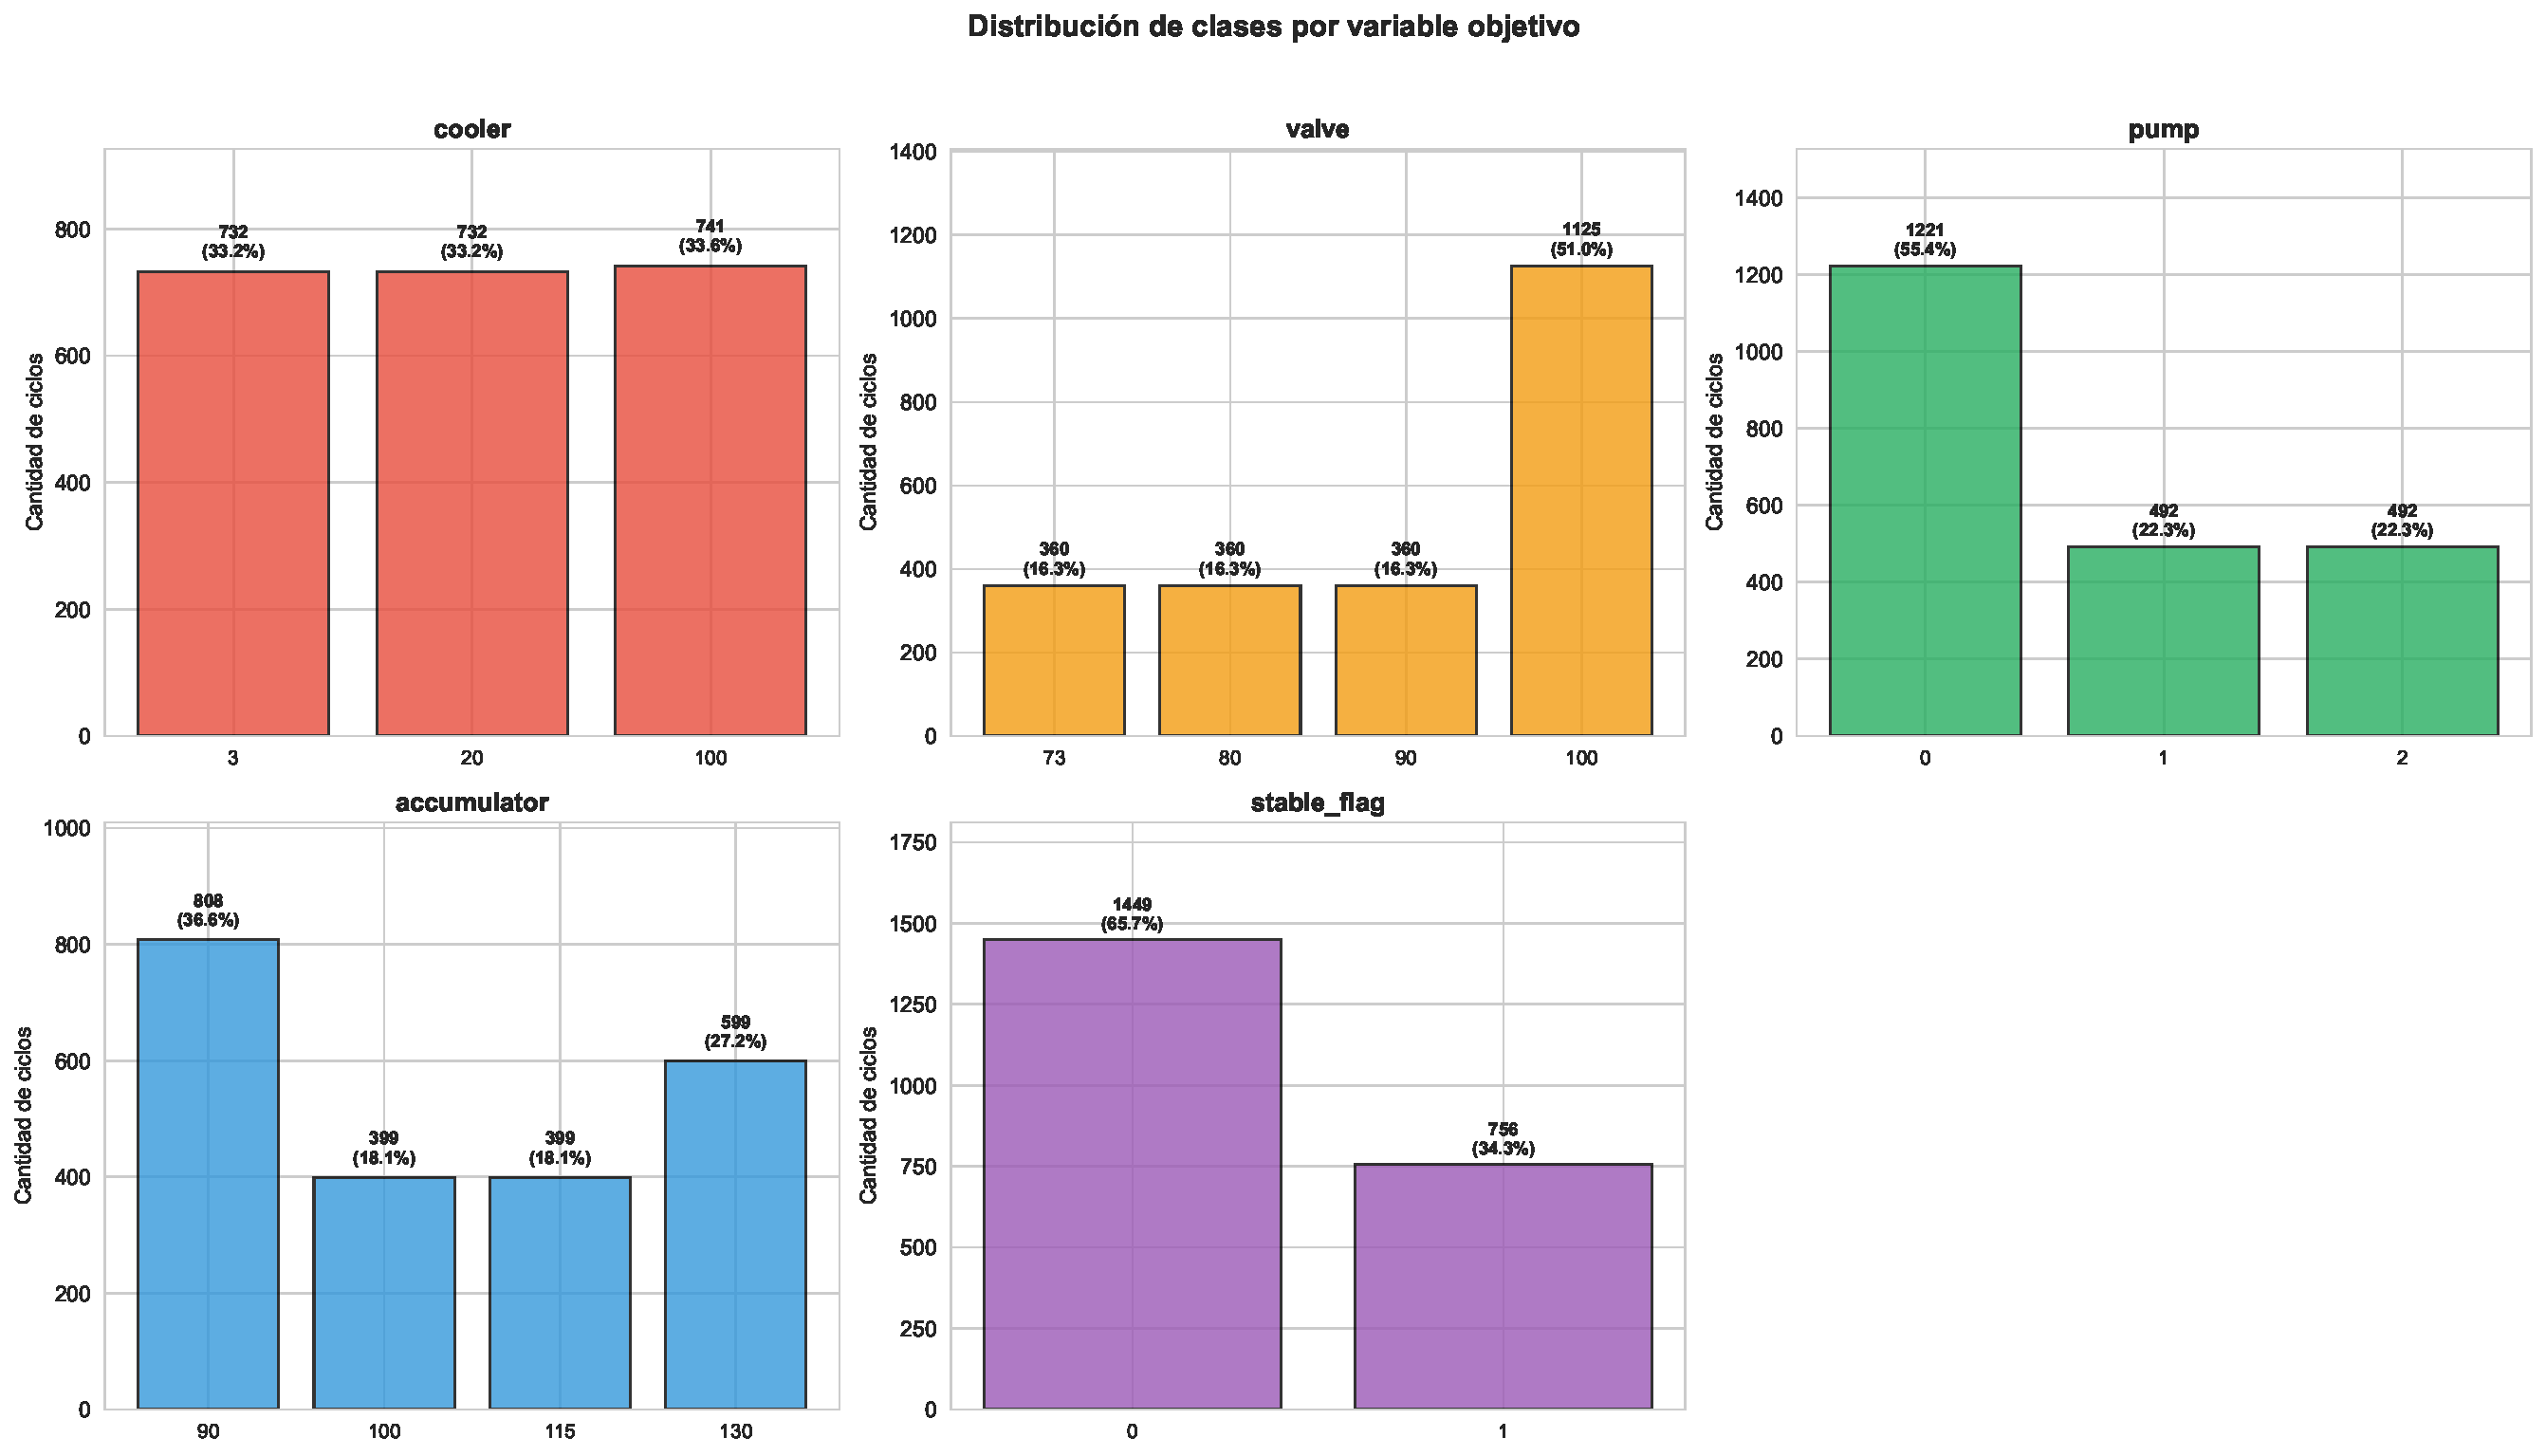
\includegraphics[width=\columnwidth]{figures/fig_targets_distribution.pdf}
    \caption{Distribución de clases de las variables objetivo empíricas calculadas en el dataset ZeMA.}
    \label{fig:targets_distribution}
\end{figure}

\subsection{El riesgo crítico de Data Leakage temporal}
\label{subsec:leakage}

Un aspecto fundamental detectado en el EDA, respaldado por el análisis de expertos en mantenimiento predictivo, es la correlación secuencial de los datos. Las 2\,205 ejecuciones corresponden a ciclos cronológicos consecutivos. Los estados de degradación se indujeron en bloques sostenidos de decenas o cientos de ciclos contiguos.

En un sistema hidráulico real, la temperatura y la degradación mecánica exhiben una inercia física considerable. Los ciclos inmediatamente sucesivos (e.g., ciclo $t$ y ciclo $t+1$) poseen dinámicas y perfiles de ruido cuasi idénticos. 

\begin{figure}[t]
    \centering
    \fbox{\parbox{0.92\columnwidth}{\small
    \textbf{Principio de Partición Causal en Mantenimiento:}\\
    En entornos industriales de producción continua, un algoritmo de mantenimiento nunca tiene acceso a estados futuros de degradación para diagnosticar el presente. Cualquier evaluación realista debe basarse en un corte temporal estricto: entrenar con la historia pasada ($\tau \le T_{\text{split}}$) y validar sobre la operación futura ($\tau > T_{\text{split}}$).
    }}
\end{figure}

Si se aplicase una validación cruzada estratificada con barajado aleatorio (\emph{random shuffle}), el conjunto de entrenamiento contendría copias casi exactas de las instancias de validación. Esto ocasionaría un fenómeno masivo de \textbf{Data Leakage temporal}, inflando las métricas artificialmente hacia valores cercanos al 100\% que colapsarían al desplegar el modelo en producción. Por tal motivo, se adopta como directriz central de este trabajo una \textbf{partición temporal cronológica (75\% train / 25\% test)}, complementada internamente con esquemas de validación temporal sin solapamiento hacia el futuro (\emph{TimeSeriesSplit} / bloques cronológicos). La Fig.~\ref{fig:temporal_evolution} evidencia empíricamente la estructura en bloques de fallo y el corte estricto implementado.

\begin{figure}[!t]
    \centering
    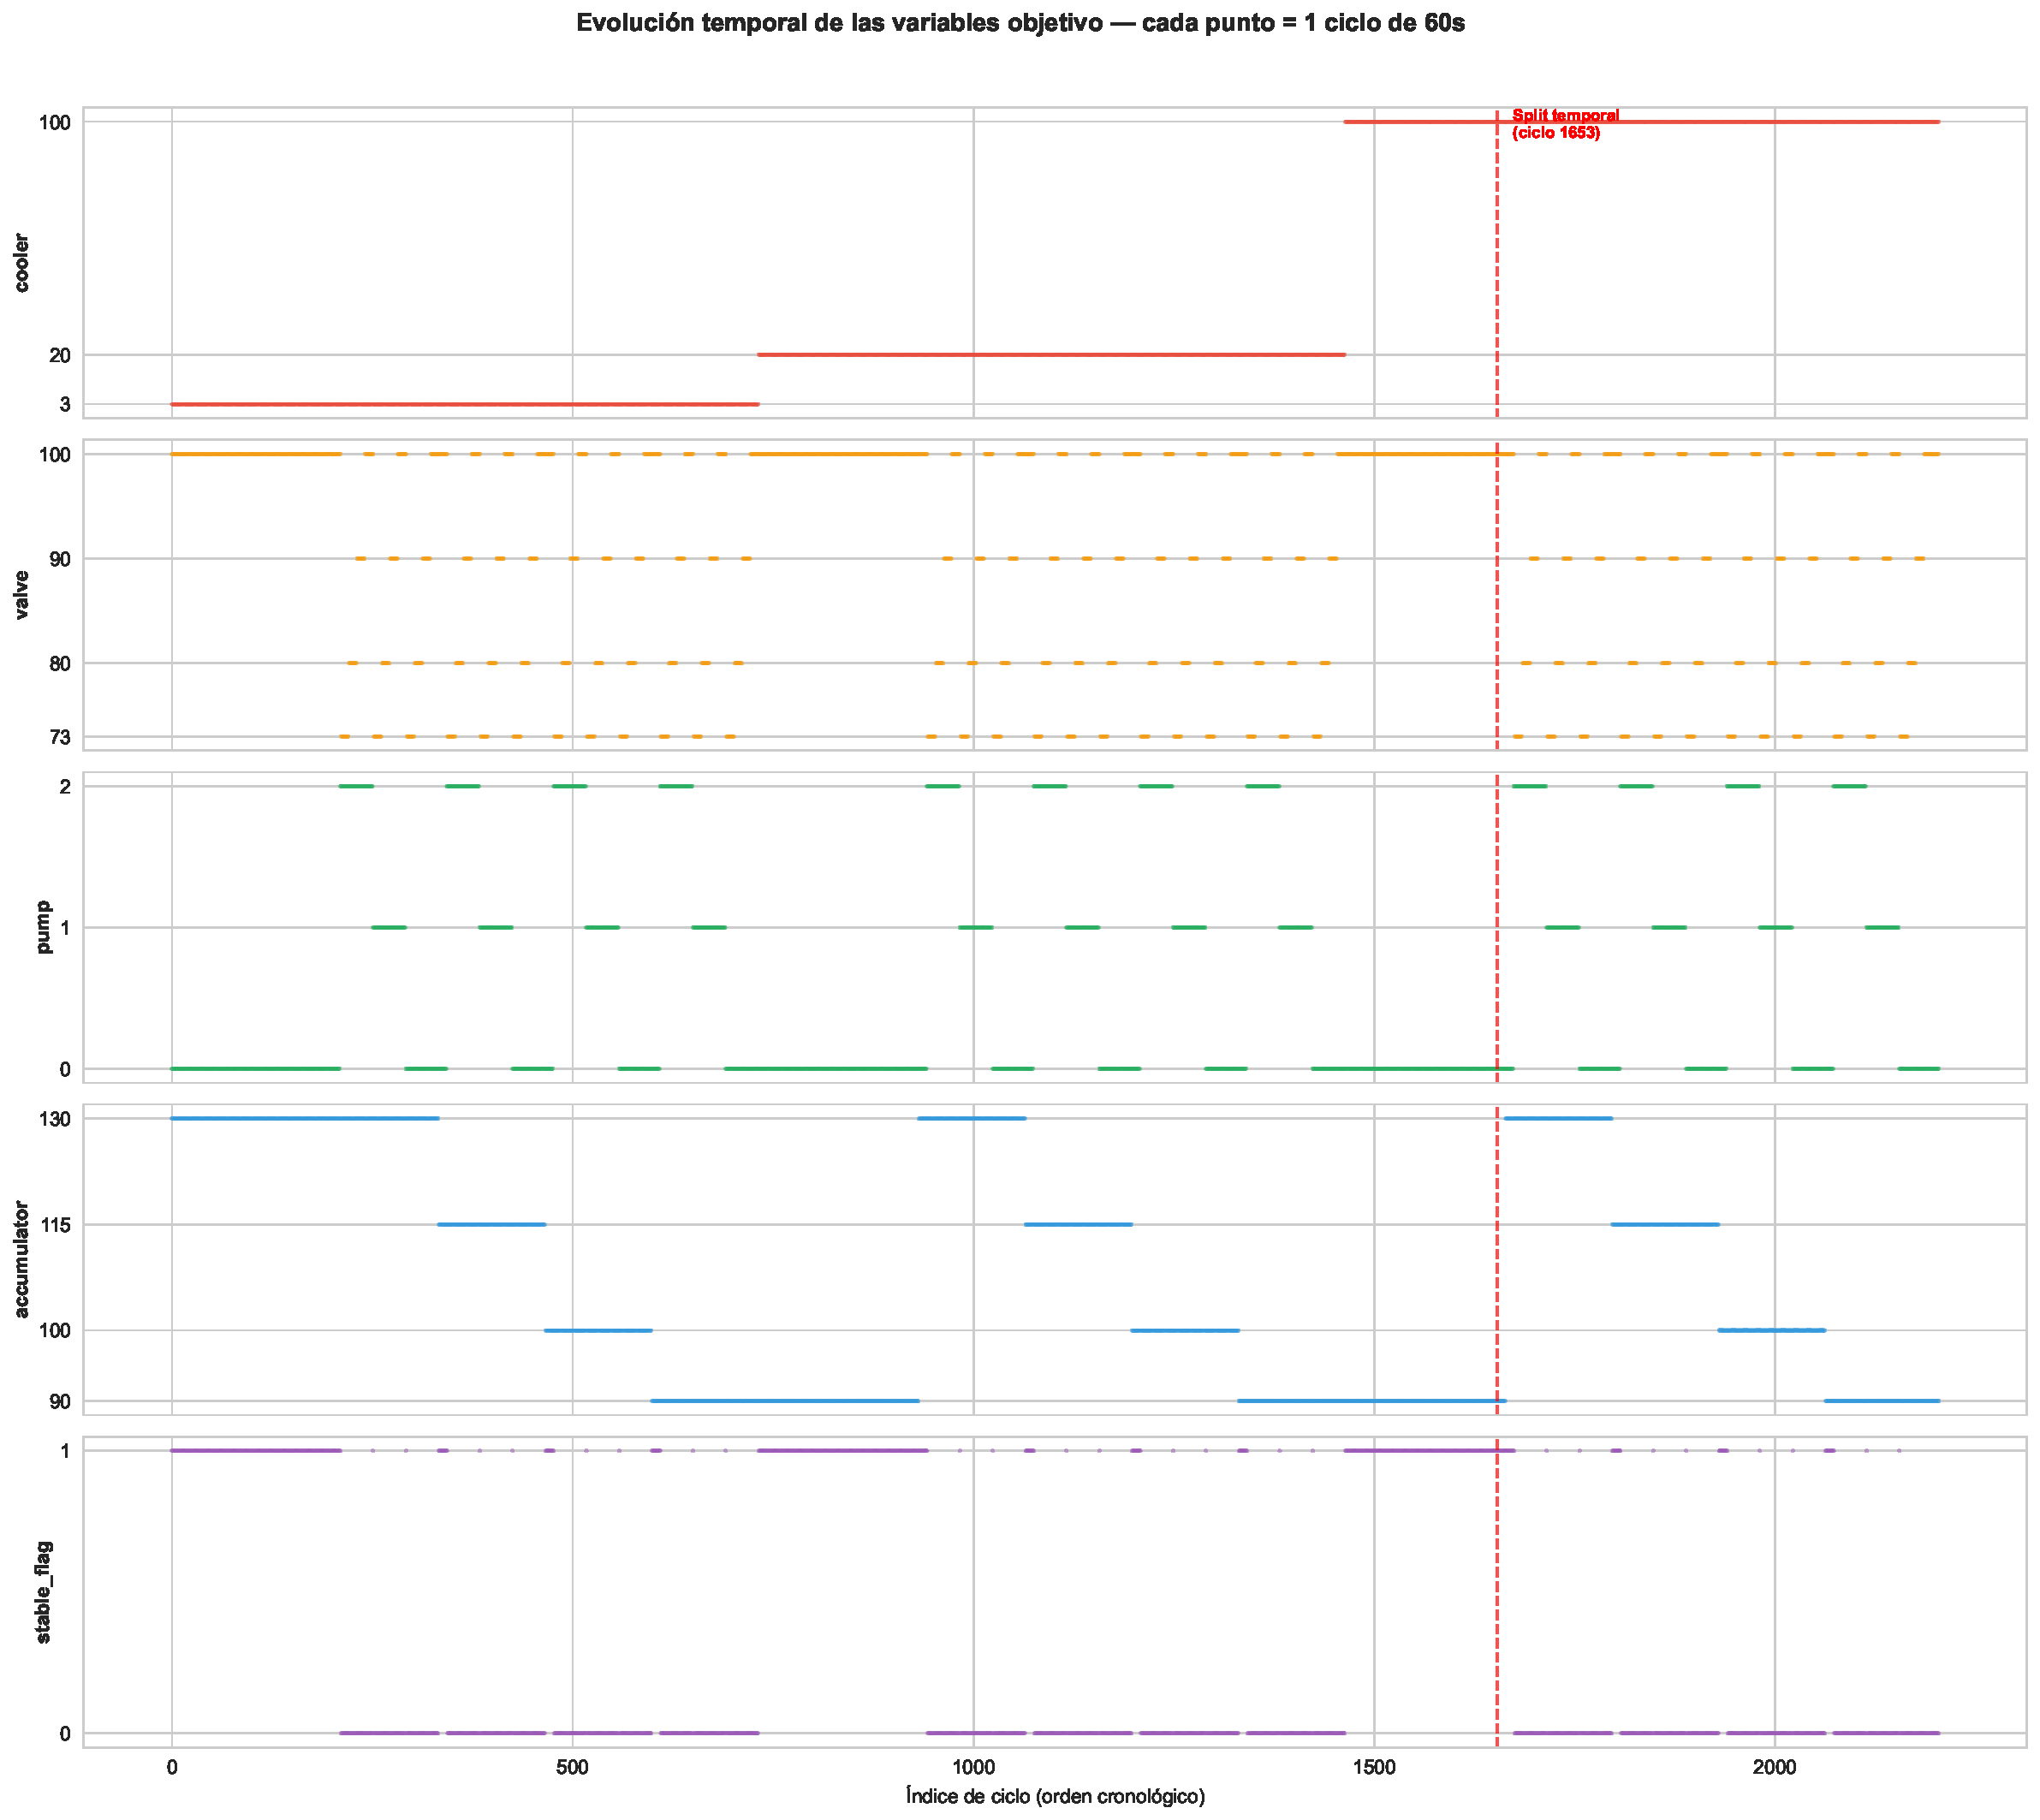
\includegraphics[width=\columnwidth]{figures/fig_temporal_evolution.pdf}
    \caption{Evolución cronológica de las 5 condiciones del perfil a lo largo de los 2\,205 ciclos de trabajo, ilustrando la estructura en bloques de fallo y el corte del split temporal al 75\% (ciclo 1\,653, línea discontinua roja).}
    \label{fig:temporal_evolution}
\end{figure}

\subsection{Inspección física de señales y contrastación preliminar}

El trazado de señales ciclo-a-ciclo para sensores representativos (Fig.~\ref{fig:sample_signals}) y el análisis de distribuciones por ciclo mediante diagramas de caja (Fig.~\ref{fig:boxplots_eda}) corroboran las hipótesis H1 y H2:

\begin{figure*}[!t]
    \centering
    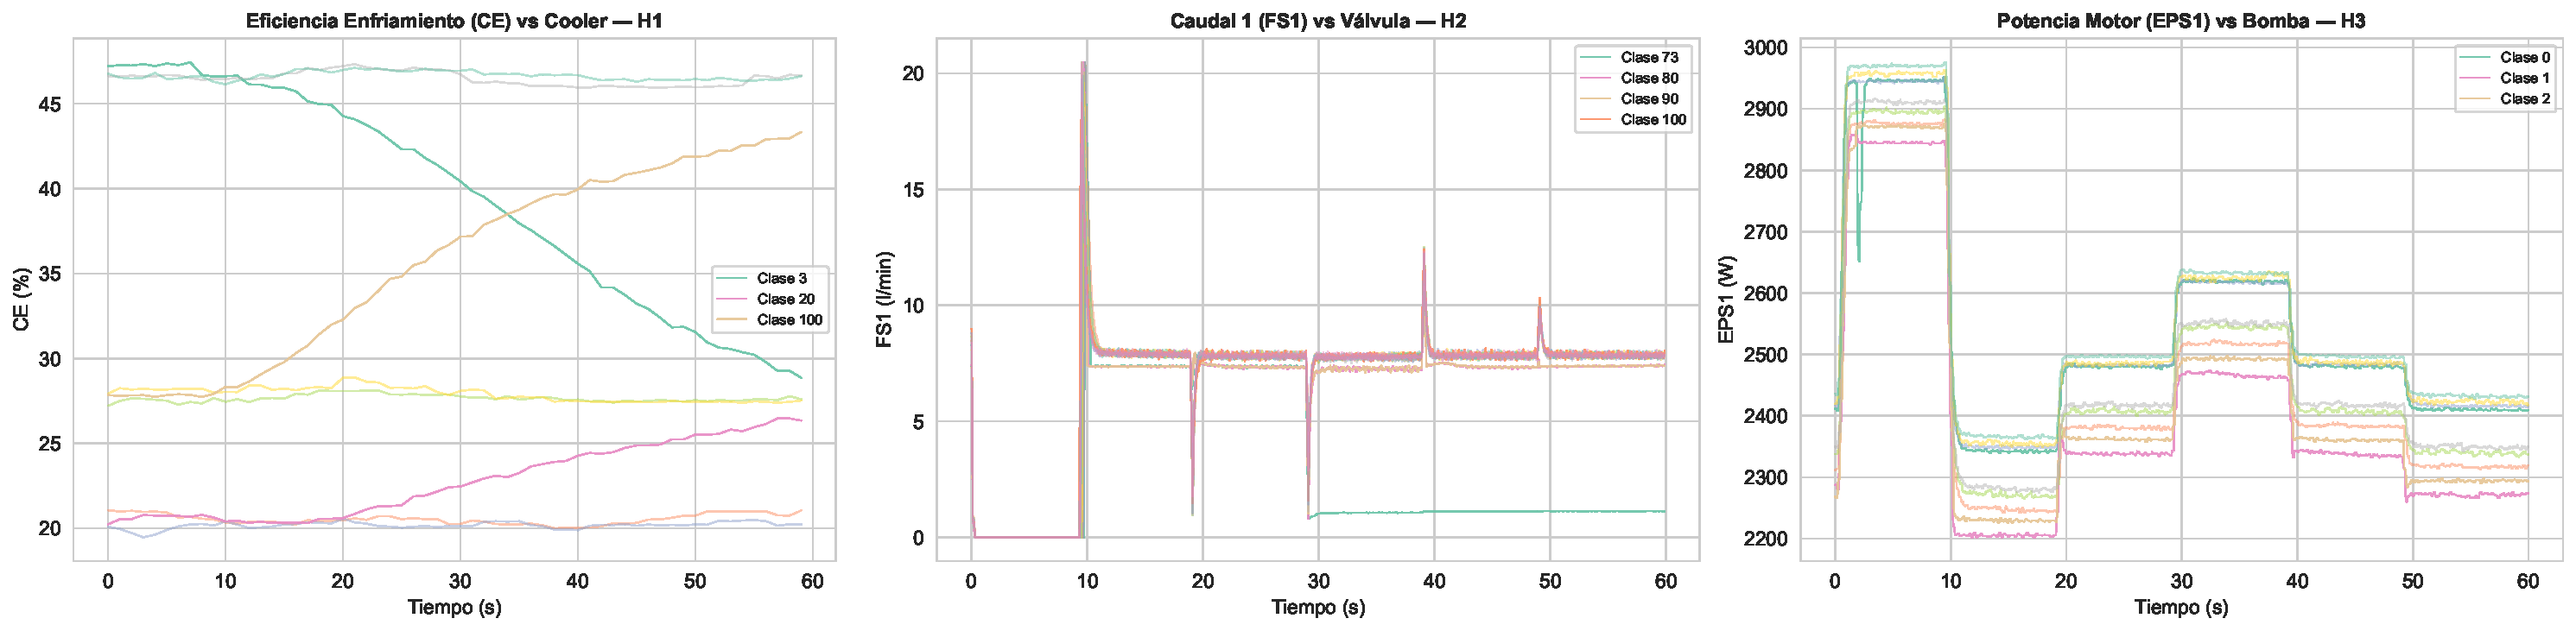
\includegraphics[width=0.95\textwidth]{figures/fig_sample_signals.pdf}
    \caption{Comportamiento transitorio de señales crudas representativas durante ciclos de \SI{60}{\second} según condición de falla: eficiencia $\text{CE}$ vs. Refrigerador (H1), caudal $\text{FS1}$ vs. Válvula (H2), y potencia $\text{EPS1}$ vs. Bomba (H3).}
    \label{fig:sample_signals}
\end{figure*}

\begin{figure*}[!t]
    \centering
    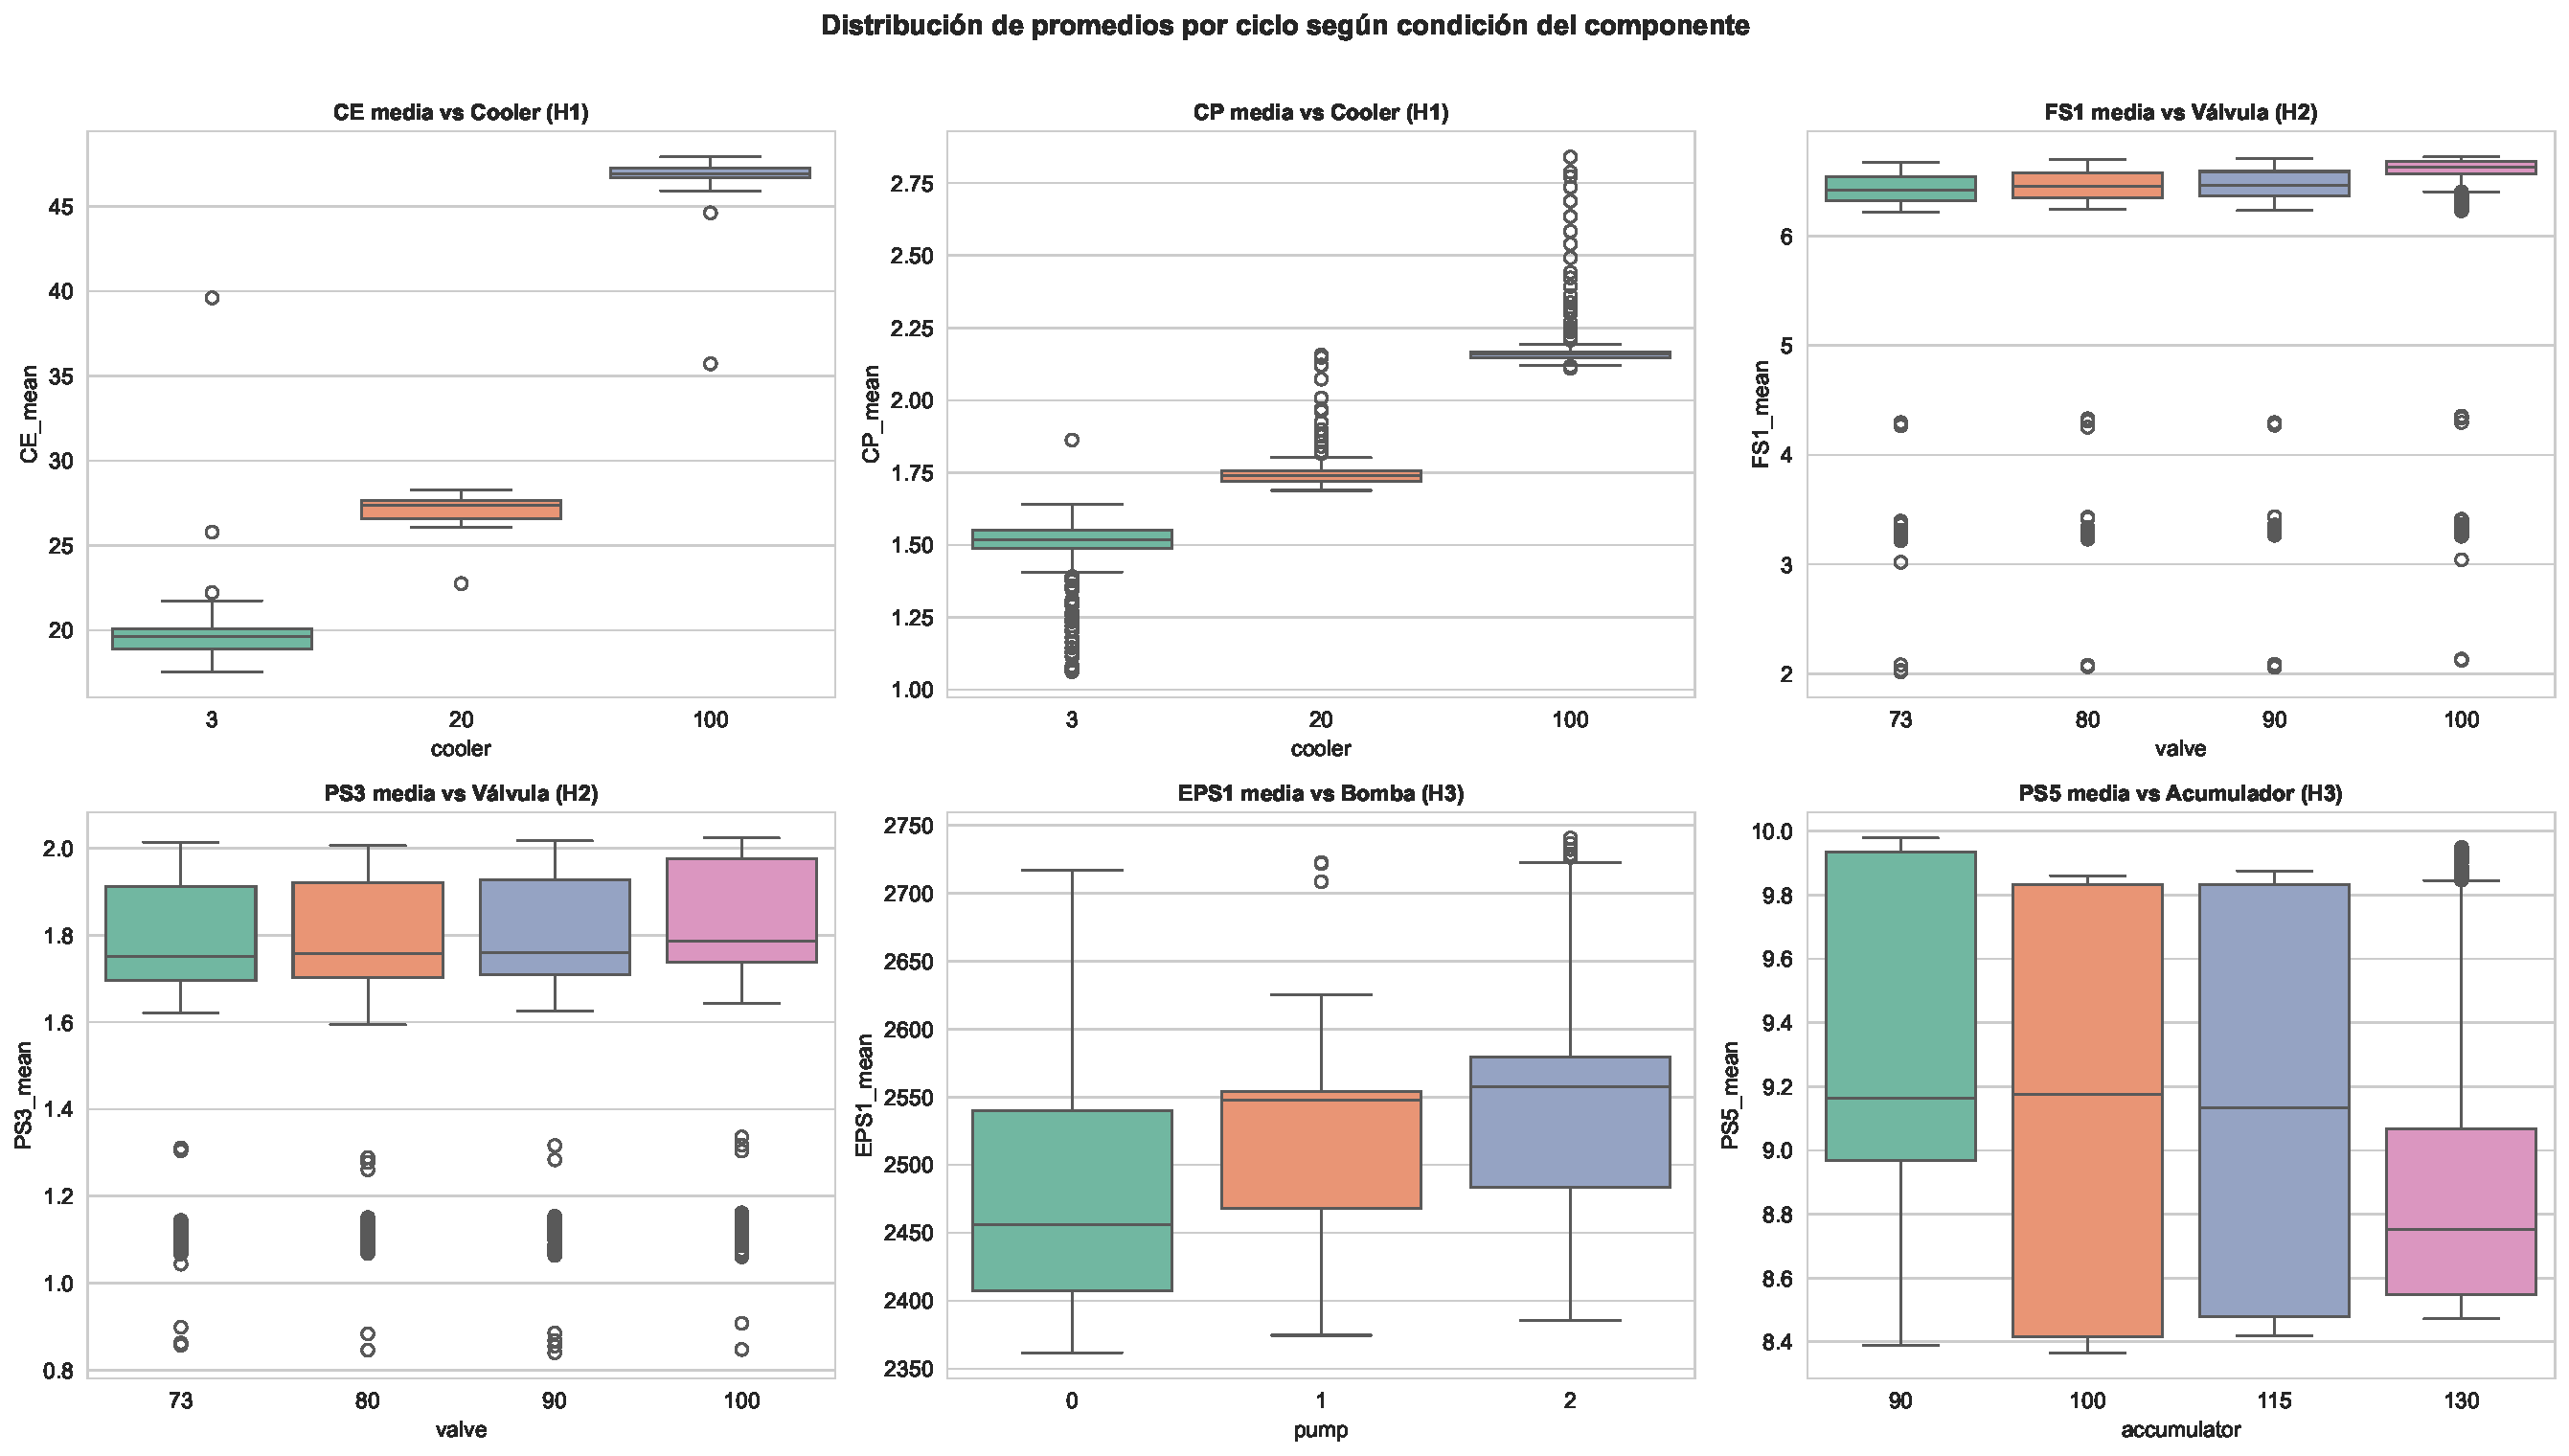
\includegraphics[width=0.95\textwidth]{figures/fig_boxplots_eda.pdf}
    \caption{Diagramas de caja (\emph{boxplots}) de promedios por ciclo para pares sensor-target según las hipótesis H1--H3, evidenciando empíricamente la separabilidad de clases para el diseño del \emph{baseline} heurístico.}
    \label{fig:boxplots_eda}
\end{figure*}
\begin{enumerate}[leftmargin=*]
    \item \textbf{Validación visual de H1:} Los sensores virtuales $\text{CE}$ (eficiencia de enfriamiento) y $\text{CP}$ (potencia disipada) caen drásticamente en saltos discretos al transicionar entre 100\%, 20\% y 3\%, evidenciando una separabilidad casi lineal respecto al refrigerador.
    \item \textbf{Validación visual de H2:} El caudal $\text{FS1}$ exhibe variaciones dinámicas en su meseta y pendiente de respuesta durante las maniobras de la válvula.
    \item \textbf{Observación sobre H3:} En contraposición, las señales de presión del acumulador y fuga de bomba están moduladas por la temperatura fluctuante del aceite, lo que difumina las fronteras de decisión y confirma que serán los objetivos más complejos de clasificar, tal como anticiparon Helwig et al.~\cite{Helwig2015}.
\end{enumerate}

% ============================================================================
% 4. INGENIERÍA DE CARACTERÍSTICAS
% ============================================================================
\subsection{Matriz de correlación sensorial}
La Fig.~\ref{fig:correlation_heatmap} presenta la correlación de Pearson entre los promedios por ciclo de los 17 sensores, evidenciando el acoplamiento multifísico (presiones entre sí, temperaturas térmicamente ligadas y variables virtuales).

\begin{figure}[!t]
    \centering
    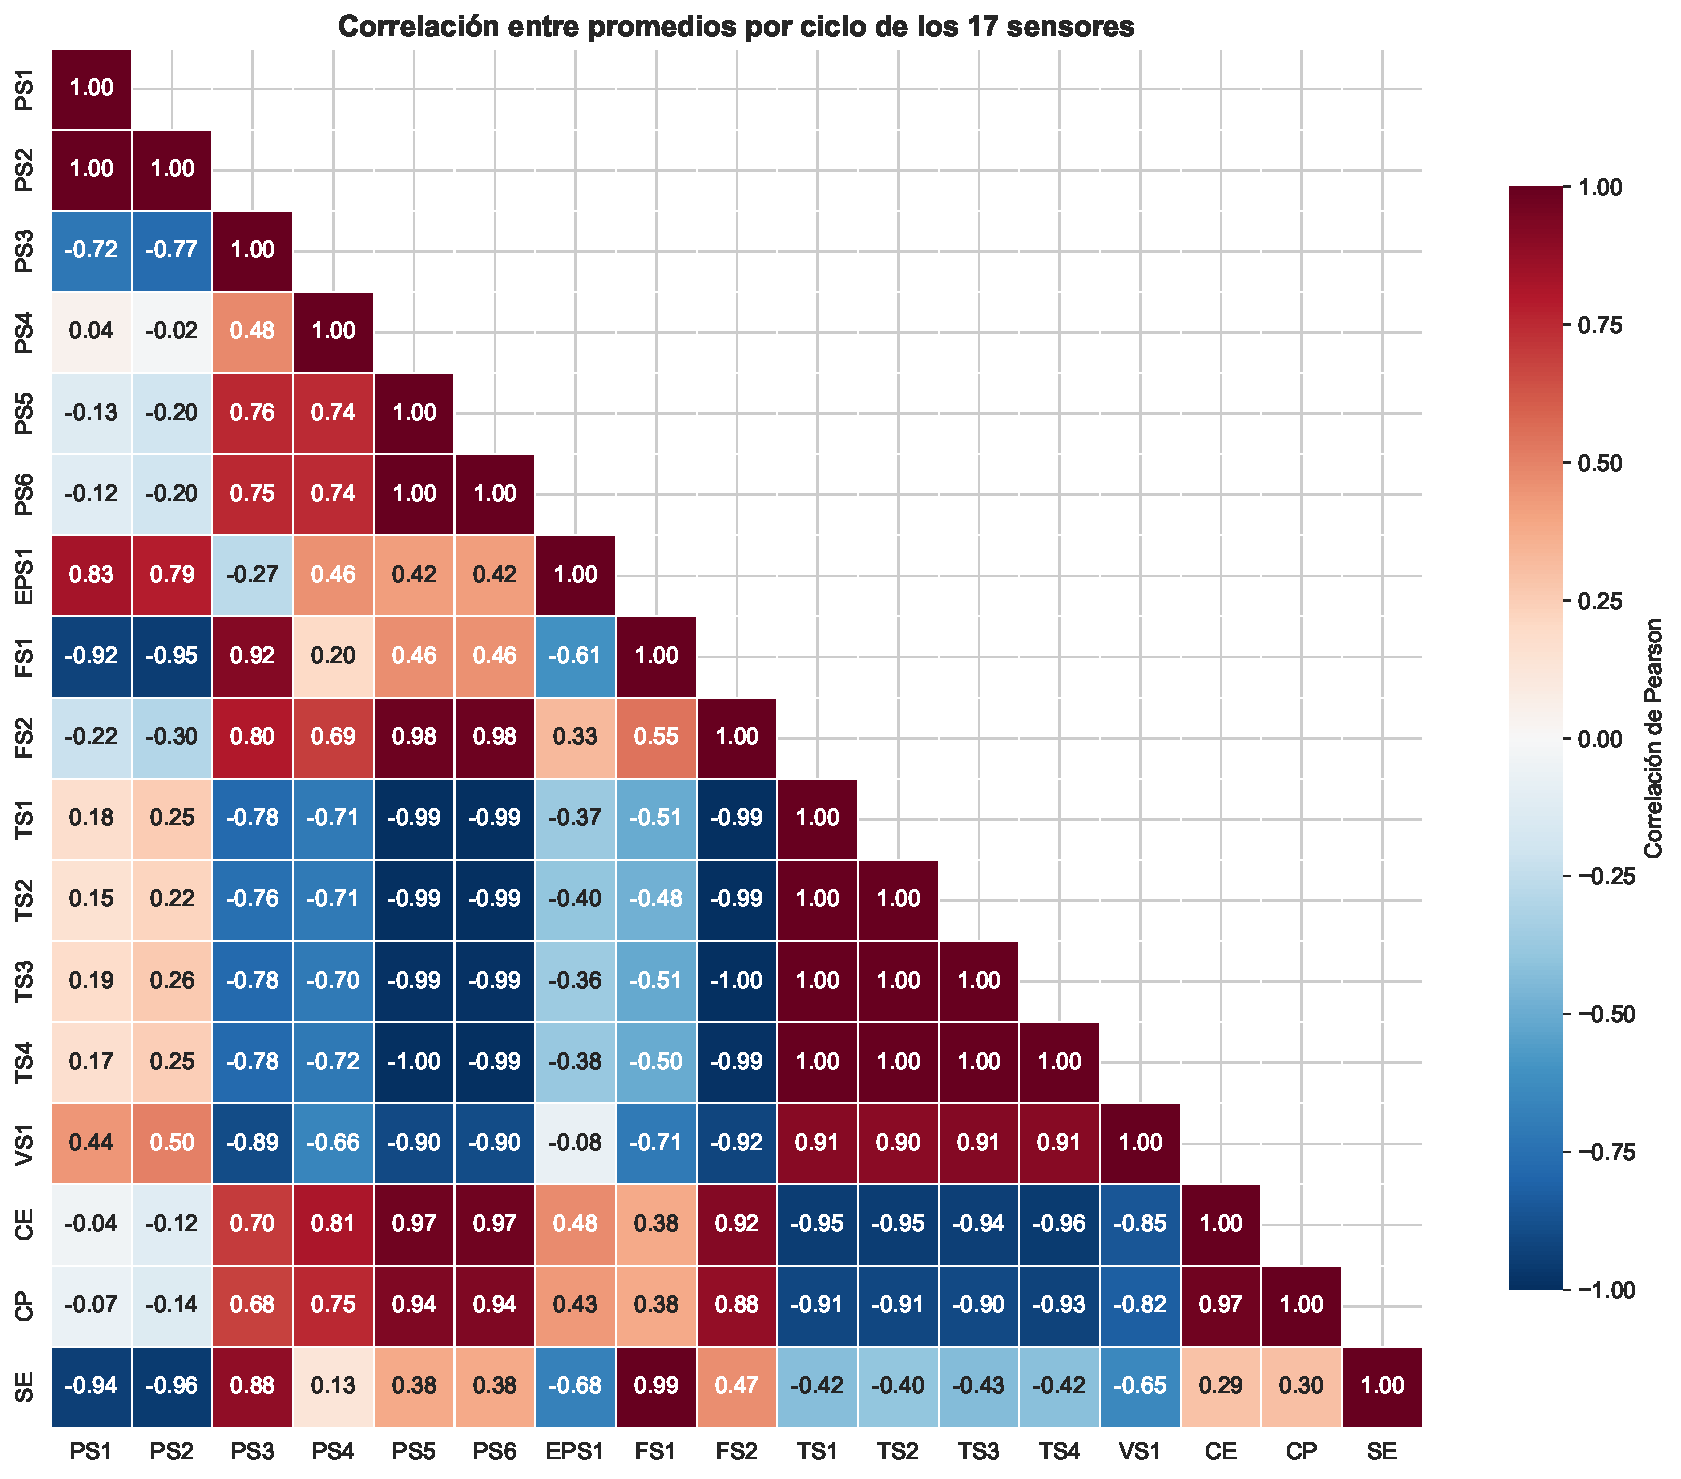
\includegraphics[width=\columnwidth]{figures/fig_correlation_heatmap.pdf}
    \caption{Matriz de correlación de Pearson entre los promedios por ciclo de los 17 canales de medición.}
    \label{fig:correlation_heatmap}
\end{figure}

\section{Ingeniería de Características}
\label{sec:features}

\subsection{Justificación de la reducción dimensional}

Entrenar clasificadores tabulares clásicos (KNN, SVM, Árboles) directamente sobre el espacio crudo de $\mathbb{R}^{43\,680}$ incurre en la \emph{maldición de la dimensionalidad}: las distancias euclidianas se vuelven equiprobables, el sobreajuste es inminente y los requerimientos de memoria y tiempo computacional crecen de forma intolerable.

Siguiendo la metodología de extracción sistemática propuesta por Schneider et al.~\cite{Schneider2017} y Helwig et al.~\cite{Helwig2015}, se opta por transformar cada serie de tiempo unidimensional $s(t)$ de duración $N$ muestras en un vector compacto de \textbf{12 descriptores estadísticos y morfológicos}.

\subsection{Formulación matemática de descriptores}

Para cada sensor $k \in \{1, \dots, 17\}$ y cada ciclo $c \in \{1, \dots, 2\,205\}$, con señal discreta $x = (x_1, x_2, \dots, x_N)$, se calculan:

\begin{enumerate}[leftmargin=*]
    \item \textbf{Media aritmética ($\mu$):}
    \begin{equation}
        \mu = \frac{1}{N}\sum_{i=1}^N x_i
    \end{equation}
    \item \textbf{Desviación estándar ($\sigma$):}
    \begin{equation}
        \sigma = \sqrt{\frac{1}{N}\sum_{i=1}^N (x_i - \mu)^2}
    \end{equation}
    \item \textbf{Mínimo y Máximo:}
    \begin{equation}
        x_{\min} = \min_{1 \le i \le N} x_i, \quad x_{\max} = \max_{1 \le i \le N} x_i
    \end{equation}
    \item \textbf{Rango pico a pico:}
    \begin{equation}
        R = x_{\max} - x_{\min}
    \end{equation}
    \item \textbf{Cuantiles empíricos ($Q_p$):} Calculados para $p \in \{0.10, 0.25, 0.50, 0.75, 0.90\}$, donde $Q_{0.50}$ representa la mediana robusta ante impulsos.
    \item \textbf{Valor cuadrático medio (RMS):} Indicador clave de energía de la señal:
    \begin{equation}
        \text{RMS} = \sqrt{\frac{1}{N}\sum_{i=1}^N x_i^2}
    \end{equation}
    \item \textbf{Pendiente de tendencia lineal ($\beta$):} Estimación rápida de la deriva intra-ciclo:
    \begin{equation}
        \beta = \frac{x_N - x_1}{N \cdot \Delta t}
    \end{equation}
\end{enumerate}

Este proceso mapea el tensor crudo de entrada a una matriz tabular homogénea de dimensiones:
\begin{equation}
    \mathbf{X} \in \mathbb{R}^{2\,205 \times 204} \quad (17 \text{ sensores} \times 12 \text{ características})
\end{equation}
reduciendo el volumen dimensional en un \textbf{99.53\%} sin pérdida de las propiedades de distribución fundamentales.

\subsection{Estrategia de gestión de memoria (\emph{Process-and-Discard})}

La carga simultánea de las matrices en precisión flotante doble (\texttt{float64}) consumiría más de \SI{1.5}{\giga\byte} de RAM únicamente en matrices brutas. Para optimizar el pipeline, se instrumentó un esquema secuencial:
\begin{enumerate}
    \item Carga en precisión simple (\texttt{float32}) por canal.
    \item Extracción vectorializada de las 12 características.
    \item Liberación explícita de memoria del tensor crudo antes de procesar el siguiente canal mediante recolección de basura (\texttt{gc.collect()}).
\end{enumerate}
El dataset consolidado resultante ocupa únicamente $\approx$\SI{3.6}{\mega\byte}, permitiendo entrenamientos ultrarrápidos y reproducibilidad garantizada en cualquier estación de trabajo convencional.

\subsection{Mejoras potenciales en el dominio frecuencial}

Tal como señalan Schneider et al.~\cite{Schneider2017}, los transitorios de degradación del acumulador y las vibraciones mecánicas ($\text{VS1}$) pueden contener información confinada en el espectro armónico. Si los modelos tabulares temporales mostrasen rendimientos subóptimos en la Fase 3, se incorporará la Transformada Rápida de Fourier (FFT) y coeficientes Wavelet de Daubechies como extensión.

% ============================================================================
% 5. METODOLOGÍA DE EVALUACIÓN Y MODELADO
% ============================================================================
\section{Metodología de Evaluación y Modelado}
\label{sec:metodologia}

\subsection{Esquema de partición temporal}
\label{subsec:split_metodo}

Para dar cumplimiento estricto a las exigencias contra el data leakage (Sección~\ref{subsec:leakage}), los $2\,205$ ciclos se ordenan por su índice temporal nativo. Se establece un punto de corte cronológico al 75\%:
\begin{itemize}[leftmargin=*]
    \item \textbf{Conjunto de Entrenamiento ($\mathcal{D}_{\text{train}}$):} Ciclos $1$ al $1\,653$ ($75\%$).
    \item \textbf{Conjunto de Test Congelado ($\mathcal{D}_{\text{test}}$):} Ciclos $1\,654$ al $2\,205$ ($25\%$).
\end{itemize}

El conjunto de test se mantiene completamente aislado e intocado hasta la evaluación final de los modelos optimizados. Dentro de $\mathcal{D}_{\text{train}}$, la validación cruzada para ajuste de hiperparámetros se ejecuta mediante divisiones temporales secuenciales o $K$-fold sin permutación aleatoria (\texttt{shuffle=False}).

\subsection{Métricas de evaluación multiclase}

Debido a la presencia de clases minoritarias en los fallos severos de válvulas y bombas, el \emph{Accuracy} tradicional queda descartado. Se seleccionan:
\begin{enumerate}[leftmargin=*]
    \item \textbf{Balanced Accuracy (BA):} Promedio aritmético del \emph{recall} alcanzado en cada clase $k$:
    \begin{equation}
        \text{BA} = \frac{1}{K}\sum_{k=1}^K \frac{\text{TP}_k}{\text{TP}_k + \text{FN}_k}
    \end{equation}
    \item \textbf{F1-score Macro:} Media no ponderada del F1 por clase, que penaliza severamente el sacrificio de las clases minoritarias:
    \begin{equation}
        \text{F1}_{\text{macro}} = \frac{1}{K}\sum_{k=1}^K \frac{2 \cdot \text{P}_k \cdot \text{R}_k}{\text{P}_k + \text{R}_k}
    \end{equation}
    \item \textbf{Matrices de confusión y curvas ROC One-vs-Rest (OvR).}
\end{enumerate}

\subsection{Línea base heurística no algorítmica}
\label{subsec:baseline_metodo}

En cumplimiento de los criterios pedagógicos y metodológicos de la cátedra (donde se estipula enfáticamente que un \emph{baseline} no puede ser un modelo estadístico complejo como regresión logística), se diseñan reglas empíricas derivadas directamente de la física observada en el EDA:
\begin{itemize}[leftmargin=*]
    \item \textbf{Baseline Cooler:} Umbral físico sobre el promedio de eficiencia virtual $\mu(\text{CE})$:
    \begin{equation}
        \hat{y}_{\text{cooler}} = \begin{cases} 
            3\%, & \text{si } \mu(\text{CE}) < \theta_1 \\ 
            20\%, & \text{si } \theta_1 \le \mu(\text{CE}) < \theta_2 \\ 
            100\%, & \text{si } \mu(\text{CE}) \ge \theta_2 
        \end{cases}
    \end{equation}
    \item \textbf{Baseline Valve:} Umbral de caudal promedio sobre $\mu(\text{FS1})$.
    \item \textbf{Piso estadístico absoluto:} Clasificador trivial \texttt{DummyClassifier} de clase mayoritaria.
\end{itemize}

\subsection{Familias de modelos a comparar}

Se seleccionan cuatro familias algorítmicas canónicas que cubren los enfoques fundamentales de la materia:
\begin{enumerate}[leftmargin=*]
    \item \textbf{K-Nearest Neighbors (KNN)~\cite{Cover1967}:} Basado en distancias euclidianas/Manhattan. Es mandatorio empaquetar el escalador de variables dentro de un \texttt{Pipeline(StandardScaler, KNeighborsClassifier)} para impedir la fuga de escala en los pliegues de validación cruzada.
    \item \textbf{Support Vector Machines (SVM)~\cite{Cortes1995}:} Clasificador de margen máximo con ponderación equilibrada (\texttt{class\_weight='balanced'}). Se optimizan grillas disyuntas por tipo de kernel: lineal ($C$) y función de base radial RBF ($C$, $\gamma$).
    \item \textbf{Árboles de Decisión (CART):} Modelo interpretable sin escalado de variables, regularizado mediante poda por complejidad de costo (\emph{cost-complexity pruning}, \texttt{ccp\_alpha}).
    \item \textbf{Ensambles (Random Forest~\cite{Breiman2001} y XGBoost~\cite{ChenGuestrin2016}):} Métodos de reducción de varianza (bagging) y sesgo (gradient boosting). Para Random Forest se fija explícitamente \texttt{max\_features='sqrt'}, y para XGBoost se incorpora parada temprana (\emph{early stopping}) y sintonización bayesiana con Optuna~\cite{Akiba2019}.
\end{enumerate}

% ============================================================================
% 6. RESULTADOS ESPERADOS (ESQUELETO FASE 3)
% ============================================================================
\section{Resultados y Comparativa}
\label{sec:resultados}

% TODO: En Fase 3 se incorporará la tabla comparativa exhaustiva de métricas
% para todos los modelos vs el baseline heurístico en validación y test.

\subsection{Tabla comparativa de modelos}

La Tabla~\ref{tab:results_placeholder} define la estructura formal de consolidación que se completará al ejecutar las búsquedas de hiperparámetros en la Fase 3.

\begin{table}[t]
    \centering
    \caption{Estructura de la tabla comparativa (Fase 3).}
    \label{tab:results_placeholder}
    \resizebox{\columnwidth}{!}{%
    \begin{tabular}{llcccc}
        \toprule
        \textbf{Target} & \textbf{Modelo} & \textbf{BA (CV)} & \textbf{F1 (CV)} & \textbf{BA (Test)} & \textbf{F1 (Test)} \\
        \midrule
        \multirow{5}{*}{Cooler} 
        & Baseline Dummy & --- & --- & --- & --- \\
        & Baseline Heurístico & --- & --- & --- & --- \\
        & KNN (\texttt{StandardScaler}) & --- & --- & --- & --- \\
        & SVM (Kernel RBF) & --- & --- & --- & --- \\
        & Árbol Podado (\texttt{ccp\_alpha}) & --- & --- & --- & --- \\
        & Random Forest & --- & --- & --- & --- \\
        & XGBoost & --- & --- & --- & --- \\
        \midrule
        \multirow{5}{*}{Valve} 
        & Baseline Heurístico & --- & --- & --- & --- \\
        & KNN & --- & --- & --- & --- \\
        & SVM & --- & --- & --- & --- \\
        & Random Forest & --- & --- & --- & --- \\
        & XGBoost & --- & --- & --- & --- \\
        \bottomrule
    \end{tabular}%
    }
\end{table}

\subsection{Curvas ROC y análisis de importancia de atributos}

Para cada modelo finalista se graficarán las curvas ROC One-vs-Rest por clase y se extraerán las importancias relativas de las características (\emph{permutation importance} y ganancia en árboles), validando si las variables dominantes coinciden con lo previsto en las hipótesis H1 y H2.

% ============================================================================
% 7. ANÁLISIS Y SELECCIÓN DEL MODELO (ESQUELETO FASE 4)
% ============================================================================
\section{Análisis de Diagnóstico y Selección}
\label{sec:analisis}

% TODO: En Fase 4 se detallará el análisis de errores de matrices de confusión,
% justificando la elección final considerando compensaciones de negocio:
% Rendimiento vs Simplicidad vs Costo Computacional.

Se examinarán los patrones de confusión entre estados adyacentes de fallo. En caso de discrepancias o resultados modestos en los objetivos complejos, se formularán las hipótesis explicativas pertinentes, respetando el principio evaluativo de que los resultados negativos con justificación rigurosa forman parte de la madurez investigativa.

% ============================================================================
% 8. CONCLUSIONES Y TRABAJO FUTURO (ESQUELETO FASE 5)
% ============================================================================
\section{Conclusiones y Trabajo Futuro}
\label{sec:conclusiones}

% TODO: En Fase 5 se sintetizará la validación o refutación de H1-H4,
% lecciones aprendidas sobre el split temporal y líneas de investigación futuras
% (Deep Learning 1D-CNN, Wavelets, despliegue en tiempo real).

Las fases preliminares confirman que la ingeniería de características estadísticas permite comprimir de forma masiva series temporales industriales complejas preservando la capacidad diagnóstica. El reconocimiento explícito de la naturaleza cronológica de los datos y el rechazo al barajado aleatorio sientan las bases de una experimentación veraz y transferible a sistemas de producción reales.

% ============================================================================
% BIBLIOGRAFÍA
% ============================================================================
\bibliographystyle{IEEEtran}
\bibliography{references}

\end{document}
